\documentclass{tufte-handout}
\usepackage{amsmath,amsthm}

\usepackage{pgfplots}
\pgfplotsset{width=\textwidth,compat=1.5.1}

\newtheorem{claim}{Claim}[section]
\title{\sf Approximation Algorithm for Maximum Cut}
%\date{\GITAuthorDate}
%\author{Thore Husfeldt}
% just checking how github works

\begin{document}
\maketitle

\section{Maxcut Lab Report}
by Erik Westrup and Dmitry Basavin.

\subsection{Running time}

The running time of algorithm~R is $[\ldots]$.

\subsection{Randomness}

Algorithm R uses $[\ldots]$ random bits.

\subsection{Solution quality}

\paragraph{Experiments.}

\begin{enumerate}
\item
For the input file  pw09\_100.9.txt with $t=100$ runs, we found
an average cutsize of $C=[\ldots]$, roughly $[\ldots]$\% of the optimum
$\operatorname{OPT} = 13658$.
The distribution of cutsizes looks as follows:

\medskip

\noindent
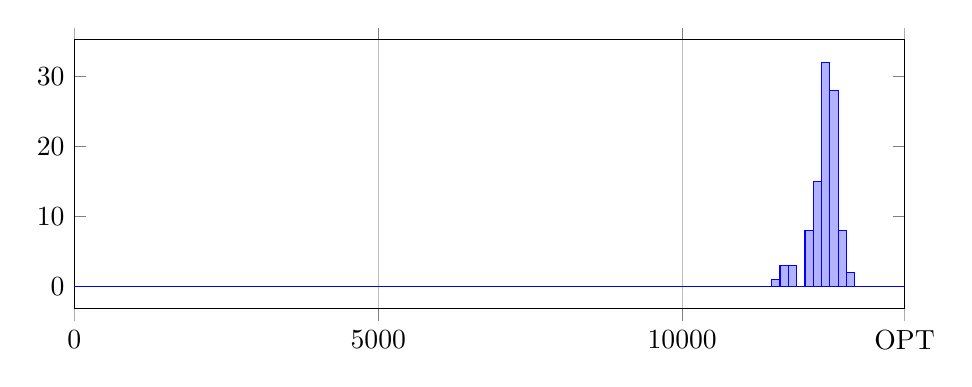
\begin{tikzpicture}
\begin{axis}[
  height= 5cm,
  ybar interval,
  xmin = 0,  xmax = 13658,
  xtick =       {0   ,   5000,   10000, 13658},
  xticklabels = { $0$, $5000$, $10000$,   OPT},
  x tick label as interval = false,
  scaled ticks = false
]
    \addplot+[hist={bins=100}]
        table[y index=0] {
          % output of 
          % perl -e "for $i (1..100) { system 'python sol/rmaxcut.py < data/pw09_100.9.txt '}"
12296
12401
12176
12414
11767
12458
12407
12551
12363
12526
11865
12353
12159
12504
12130
11616
12347
12201
12473
12368
12196
12274
12064
12398
12733
12620
12402
12231
12442
12360
12567
11650
12334
12543
12108
12523
12256
12524
12642
12040
12404
12408
12606
12094
12484
12457
12459
12326
12307
12282
12276
12459
12107
12474
12410
12109
12308
12471
12588
12473
12338
12499
12233
12453
12448
12541
12488
12497
12230
12393
12335
12446
11503
12304
12612
12378
12108
12684
12422
12557
12441
12334
12400
12369
11734
12237
12631
12289
11773
12460
12366
12355
12502
12323
12543
12271
12415
12227
12711
12370
    };
\end{axis}
\end{tikzpicture}

\item
For the input file matching\_1000.txt
$[\ldots]$
\end{enumerate}
\paragraph{Analysis of performance guarantee}

Clearly, Algorithm R performs quite badly on input 
  matching\_1000.txt.
We will show that it can perform \emph{no worse} than that, i.e., we
will establish that in expectation, the cutsize $C$ satisfies $C \geq
[\ldots]\cdot \operatorname{OPT}$.\


We will view $C$ as a random variable that gives the size of the cut
defined by the random choices.
Let $W$ denote the total weight of the edges of $G$, i.e.,
\[ W= \sum_{e\in E} w(e)\,.\]

Then,
\begin{equation}\label{eq: E[C]}
E[C] = \textstyle\frac{1}{2}\cdot W\,.
\end{equation}

To see this, define the indicator random variable $X_{uv}$ for every
edge $uv\in E$ as follows.
Set $X_{uv}=1$ if $uv$ crosses the cut, i.e., $u\in A$ and $v\notin A$
or $u\notin A$ and $v\in A$.
Otherwise, $X_{uv} = 0$.

Then, $\Pr(X_{uv} = 1) = [\ldots]$.
Now, $E[C]=[\ldots]$ Finally, we have 
\(E[C]\geq [\ldots]\cdot \text{OPT}\) because clearly
$[\ldots]$.


\end{document}
